% !TEX encoding = UTF-8 Unicode
% CDSL@UoS template: 4:3, boxes, 10pt, serif math, original logos and margins.
\documentclass[t,10pt,handout]{beamer}
% Original CDSL@UoS preamble, with class/note mode in main.tex.
% This is a basic template for H. Shim
% Aug. 19, 2008
% Modified by G. Park
% Sept. 20, 2023

% 제출해야할 때 handout 옵션 추가 발표할 때는 제거. 발표할 때 \pause 효과를 사용 할 수 있게 됨


  
\def\mynote{aa}   % Comment if mynote wants to appear

\mode<presentation>
{
  \usetheme{boxes}
  \usefonttheme[onlymath]{serif}
  \setbeamercovered{transparent}
}

\setbeamertemplate{navigation symbols}{}
% removes the navigation symbols
\setbeamertemplate{footline}[frame number]
%\setbeamertemplate{footline}[text line]{%
%color setting more or less matching U of A colors
%\setbeamercolor*{palette secondary}{use=structure,fg=white,bg=structure.fg!55!black}
%\setbeamercolor*{palette tertiary}{use=structure,fg=white,bg=red!50!black}

\usepackage{kotex}
\usepackage[english]{babel}
\usepackage[T1]{fontenc}
\usepackage{comment}
\usepackage{mathtools}
\usepackage{setspace}

\colorlet{Darkred}{red!50!black}
\colorlet{Darkgreen}{green!50!black}
\colorlet{Darkblue}{blue!70!black}
\newcommand{\colb}{\color{Darkblue}}
\newcommand{\colgr}{\color{gray}}
\newcommand{\colg}{\color{Darkgreen}}
\newcommand{\colr}{\color{Darkred}}

% Define Environment:
\newtheorem{thm}{\bf Theorem}
\newtheorem{prop}{\bf Proposition}
\newtheorem{lem}{\bf Lemma}
\newtheorem{assmpt}{\bf Assumption}
\newtheorem{defn}{\bf Definition}
\newtheorem{exmp}{\bf Example}
\newtheorem{cor}{\bf Corollary}
\newtheorem{condi}{\bf Condition}
%=== Non-italic Theorem Environment by Vin
\newtheorem{rem1}{\bf Remark}
\newenvironment{rem}{\begin{rem1}\normalfont}{\end{rem1}}
%=== New Example Environment by Vin
\newcounter{Examp}
\newenvironment{exam}{\stepcounter{Examp} \medskip \noindent {\bf Example \arabic{Examp}.}}{ \medskip }

%=== New Example Environment by Vin
\newcounter{exer}
\newenvironment{exer}{\stepcounter{exer} \medskip \noindent {\bf Exercise \arabic{exer}.}}{ \medskip }


% Define Some Notation:

\newcommand{\nn}{{\mathfrak{n}}}

\newcommand{\R}{\ensuremath{{\mathbb R}}}
\newcommand{\Z}{\ensuremath{{\mathbb Z}}}
\newcommand{\N}{\ensuremath{{\mathbb N}}}

\newcommand{\AAA}{{\mathcal A}}
\newcommand{\CC}{{\mathcal C}}
\newcommand{\DD}{{\mathcal D}}
\newcommand{\EE}{{\mathcal E}}
\newcommand{\FF}{{\mathcal F}}
\newcommand{\KK}{{\mathcal K}}
\newcommand{\LL}{{\mathcal L}}
\newcommand{\MM}{{\mathcal M}}
\newcommand{\NN}{{\mathcal N}}
\newcommand{\OO}{{\mathcal O}}
\newcommand{\PP}{{\mathcal P}}
\newcommand{\QQ}{{\mathcal Q}}
\newcommand{\RR}{{\mathcal R}}
\newcommand{\SSS}{{\mathcal S}}
\newcommand{\TT}{{\mathcal T}}
\newcommand{\UU}{{\mathcal U}}
\newcommand{\VV}{{\mathcal V}}
\newcommand{\WW}{{\mathcal W}}
\newcommand{\XX}{{\mathcal X}}
\newcommand{\YY}{{\mathcal Y}}
\newcommand{\cN}{\ensuremath{\mathcal{N}}}

\newcommand{\KL}{{\mathcal{KL}}}
\newcommand{\sat}{\ensuremath{{\rm sat}}}

\newcommand{\triend}{\hfill \ensuremath{\lhd}}
\DeclareMathOperator{\rank}{rank}

\newcommand{\cvector}[1]{\left(\!\!\!\begin{array}{c} #1 \end{array}\!\!\!\right)}
\newcommand{\setdef}[2]{\left\{\ #1\ \left|\ #2\ \right.\right\}}

\setbeamertemplate{itemize subitem}[circle]

\setstretch{1.1}

\setbeamersize{text margin left=0.5cm}  % <- like this
\setbeamersize{text margin right=0.5cm} % <- like this



\usepackage{booktabs,tabularx,bm,tikz,lmodern,appendixnumberbeamer}
\usetikzlibrary{arrows.meta,positioning,calc,fit,backgrounds,shapes.geometric}
\graphicspath{{Fig/}}
\definecolor{Accent}{HTML}{205493}
\definecolor{TitleAccent}{HTML}{26218F}
\definecolor{Success}{HTML}{28735E}
\definecolor{Muted}{HTML}{67727D}
\definecolor{Soft}{HTML}{F0F4F8}
% Saturated text emphasis, separate from structural and plot colors.
\definecolor{EmphasisRed}{HTML}{FF0000}
\definecolor{EmphasisBlue}{HTML}{0000FF}
\definecolor{EmphasisGreen}{HTML}{008000}
\definecolor{EmphasisOrange}{HTML}{E66A00}
\setbeamercolor{structure}{fg=Accent}
\setbeamercolor{block title}{fg=Soft,bg=Accent}
\setbeamercolor{block body}{fg=black,bg=Soft}
\setbeamercolor{alerted text}{fg=EmphasisRed}
\setbeamerfont{frametitle}{size=\fontsize{14.4}{17.3}\selectfont}
\setbeamerfont{title}{size=\fontsize{14.4}{17.3}\selectfont}
\setbeamerfont{subtitle}{size=\normalsize}
\setbeamerfont{framesubtitle}{size=\normalsize}
\setbeamercolor{framesubtitle}{fg=Accent}
\setbeamertemplate{bibliography item}[text]
\setbeamertemplate{bibliography entry title}{}
\setbeamertemplate{bibliography entry location}{}
\setbeamertemplate{bibliography entry note}{}
\setbeamerfont{block title}{size=\normalsize}
\setbeamertemplate{itemize item}{\color{Accent}$\blacktriangleright$}
\setlength{\tabcolsep}{5pt}
\pdfstringdefDisableCommands{\def\\{ }}

\newcommand{\takeaway}[1]{\par\begin{beamercolorbox}[sep=2mm,wd=\linewidth]{block body}\color{black}\textbf{#1}\end{beamercolorbox}\detailgap}
\newcommand{\ee}{\mathrm{ee}}
\newcommand{\qstar}{q^*}
\newcommand{\norm}[1]{\left\lVert#1\right\rVert}
\DeclareMathOperator*{\argmax}{arg\,max}
\DeclareMathOperator*{\argmin}{arg\,min}
\tikzset{box/.style={draw=Accent!60,fill=Soft,rounded corners=2pt,align=center,
    minimum height=10mm,inner sep=3mm,font=\normalsize},
    arr/.style={-{Stealth[length=2mm]},thick,draw=Accent},
    mini/.style={box,font=\normalsize,inner sep=2mm,minimum height=8mm}}

\title{3축 평면 로봇 매니퓰레이터의\\QP 기반 순차적 기구학 제어}
\subtitle{[CICS'26 Oral Session 9 : 로봇 시스템 및 제어 (1)]}
\author{\texorpdfstring{\textbf{이진우}$^1$, 박경훈$^{1,*}$,
김형종$^2$, 이승준$^2$, 최성현$^2$}{이진우, 박경훈, 김형종, 이승준, 최성현}}
\institute{\texorpdfstring{$^1$서울시립대학교,\quad
$^2$한국생산기술연구원}{서울시립대학교; 한국생산기술연구원}}
\date[2026. 11. 12.]{CICS'26 정보 및 제어 학술대회, 경주 한화리조트, 2026. 11. 12.}
\newcommand{\titlelogos}{%
\raisebox{-.5\height}{
\includegraphics[height=9mm]{CDSLlogo.png}}\hspace{4mm}%
\raisebox{-.5\height}{
\includegraphics[height=9mm]{UoSlogo.jpg}}\hspace{4mm}%
\raisebox{-.5\height}{
\includegraphics[width=34mm,height=9mm,keepaspectratio]{kitech_signature_horizontal.pdf}}}
\hypersetup{pdftitle={3축 평면 로봇 매니퓰레이터의 QP 기반 순차적 기구학 제어},pdfauthor={이진우, 박경훈, 김형종, 이승준, 최성현},pdfsubject={CICS: 10분 planar 연구 발표}}
% 본문 간격 설정. 상단 진행 표시와 하단 참고문헌, 발표 노트에는 적용하지 않음.
% 자동 줄바꿈: 10pt 글자 / 13.2pt 기준선 간격.
% 같은 설명 묶음: 1mm 추가; 다른 묶음: 3mm 추가; 그림-설명: 2mm 추가.
\newlength{\SlideBodyHeight}
\setlength{\SlideBodyHeight}{57.5mm}
\newlength{\SlideDetailGap}
\setlength{\SlideDetailGap}{1mm}
\newlength{\SlideGroupGap}
\setlength{\SlideGroupGap}{3mm}
\newlength{\SlideFigureGap}
\setlength{\SlideFigureGap}{2mm}
\newlength{\SlideMathRowGap}
\setlength{\SlideMathRowGap}{1.5mm}
\newcommand{\SlideTableStretch}{1.25}
\newcommand{\detailgap}{\par\vspace{\SlideDetailGap}}
\newcommand{\groupgap}{\par\vspace{\SlideGroupGap}}
\newcommand{\figuregap}{\par\vspace{\SlideFigureGap}}
\newenvironment{slidebody}{%
  \begin{minipage}[t][\SlideBodyHeight][c]{\linewidth}%
  \setstretch{1}\fontsize{10}{13.2}\selectfont
  \setlength{\parskip}{0pt}%
  \renewcommand{\arraystretch}{\SlideTableStretch}%
}{\par\end{minipage}}

% Fixed viewport for the model and the three consecutive control stages.
\newcommand{\planarstage}[2]{%
  \begin{columns}[c,onlytextwidth]
  \column{.43\textwidth}\begin{minipage}[c][\SlideBodyHeight][c]{\linewidth}\centering
  \includegraphics[width=\linewidth]{#1}\end{minipage}
  \column{.54\textwidth}\begin{minipage}[c][\SlideBodyHeight][c]{\linewidth}\centering #2\end{minipage}
  \end{columns}}
\newcommand{\stagechain}[1]{%
  \begin{tikzpicture}[x=1mm,y=1mm]
    \foreach \i/\col in {1/EmphasisBlue,2/EmphasisOrange,3/EmphasisGreen}{%
      \ifnum\i=#1
        \node[draw=\col,fill=\col!12,rounded corners,minimum width=14mm,minimum height=7mm](q\i)at({(\i-1)*22},0){$\mathrm{QP}_{\i}$};
      \else
        \node[draw=black!35,minimum width=14mm,minimum height=7mm,rounded corners](q\i)at({(\i-1)*22},0){$\mathrm{QP}_{\i}$};
      \fi}
    \draw[arr](q1.east)--(q2.west);\draw[arr](q2.east)--(q3.west);
  \end{tikzpicture}}
% Read slide footnotes from the same .bib used by the full bibliography.
\usepackage{usebib}
\newbibfield{shortauthor}
\newbibfield{shortvenue}
\bibinput{references}
\makeatletter
% Collect each reference once per labeled frame; retain the BibTeX numbers.
% Every frame using \slidecite must have its own unique label.
\newcommand{\slide@collectreference}[1]{%
  \ifinlistcs{#1}{slide@references@\beamer@againname}{}{%
    \listcsgadd{slide@references@\beamer@againname}{#1}}}
\newcommand{\slidecite}[1]{%
  \forcsvlist{\slide@collectreference}{#1}\cite{#1}}
\newcommand{\slide@reference}[1]{%
  \noindent\hangindent=4mm\hangafter=1
  \cite{#1}\enspace
  \usebibentry{#1}{shortauthor},
  \usebibentry{#1}{title}.
  \textit{\usebibentry{#1}{shortvenue}}, \usebibentry{#1}{year}.\par}
\newcommand{\SlideReferenceFootnotes}{%
  \ifdefined\beamer@againname
    \ifcsdef{slide@references@\beamer@againname}{%
      {\color{black!45}\hrule height.2pt}\vskip1mm
      \forlistcsloop{\slide@reference}{slide@references@\beamer@againname}%
    }{}%
  \fi}
\makeatother

% Top navigation: section labels and one dot per main slide.
% Completed: filled gray. Current: larger blue. Upcoming: hollow gray.
% The cover is excluded; backup slides have an independent page count.
\makeatletter
\providecommand{\DefenseProgressStage}{}
\newcommand{\AppendixContentsText}{Appendix contents}
\newcommand{\defensepart}[1]{\gdef\DefenseProgressStage{#1}}
\newcommand{\DefenseProgressGroups}{\defense@group{Motivation}{2}{3}\defense@group{Background}{4}{7}\defense@group{Method}{8}{13}\defense@group{Results}{14}{16}\defense@group{Closing}{17}{18}}

\def\defense@label@Motivation{Motivation}
\def\defense@label@Background{Background}
\def\defense@label@Method{Method}
\def\defense@label@Results{Results}
\def\defense@label@Closing{Closing}

\newcommand{\defense@group}[3]{%
  \def\defense@width{18mm}%
  \def\defense@candidate{#1}%
  \def\defense@name{Motivation}\ifx\defense@candidate\defense@name\def\defense@width{22mm}\fi
  \def\defense@name{Background}\ifx\defense@candidate\defense@name\def\defense@width{22mm}\fi
  \def\defense@name{Learning}\ifx\defense@candidate\defense@name\def\defense@width{17mm}\fi
  \makebox[\defense@width][c]{%
    \begin{tikzpicture}[x=1mm,y=1mm,baseline=0mm]
      \path[use as bounding box] (-8.5,0) rectangle (8.5,4);
      \def\defense@candidate{#1}%
      \ifx\DefenseProgressStage\defense@candidate
        \node[anchor=base,inner sep=0pt,font=\fontsize{7.5}{9}\selectfont\bfseries,text=Accent] at (0,2.02) {\csname defense@label@#1\endcsname};
      \else
        \node[anchor=base,inner sep=0pt,font=\fontsize{7.5}{9}\selectfont,text=black!75] at (0,2.02) {\csname defense@label@#1\endcsname};
      \fi
      \foreach \defense@page in {#2,...,#3}{%
          \pgfmathsetmacro{\defense@x}{(\defense@page-(#2+#3)/2)*1.4}%
          \ifnum\defense@page<\c@framenumber
            \fill[black!55] (\defense@x,.65) circle[radius=.38];
          \else\ifnum\defense@page=\c@framenumber
              \fill[Accent] (\defense@x,.65) circle[radius=.55];
            \else
              \draw[black!45,line width=.25pt] (\defense@x,.65) circle[radius=.38];
            \fi\fi
        }%
    \end{tikzpicture}}}

\setbeamertemplate{headline}{%
  \leavevmode
  \begingroup
  \normalfont\fontsize{9}{10.8}\selectfont
  \vbox to 2.5mm{%
      \offinterlineskip
      \vskip1mm
      \hbox to \paperwidth{%
        \hskip5mm%
        \ifbeamer@inappendix
          \vrule width0pt height4mm depth0pt%
          \raisebox{1.6mm}{\makebox[\dimexpr\paperwidth-24mm\relax][l]{\hyperlink{appendix-contents}{\color{Accent}\AppendixContentsText}}}%
          \raisebox{1.6mm}{\makebox[14mm][r]{\fontsize{7}{8.4}\selectfont\color{black!75}\insertframenumber\,/\,\inserttotalframenumber}}%
        \else
          \DefenseProgressGroups%
          \raisebox{1.6mm}{\makebox[14mm][r]{\fontsize{7}{8.4}\selectfont\color{black!75}\insertframenumber\,/\,\insertmainframenumber}}%
        \fi
        \hskip5mm\hss%
      }%
      \vss
    }%
  \endgroup
}
% Fixed-height reference area keeps the body aligned on every slide.
% Reference details are the small-font exception; body text stays at 10 pt.
\setbeamertemplate{footline}{%
  \leavevmode
  \hbox to \paperwidth{\hskip5mm%
    \vbox to 9mm{%
        \hsize=\dimexpr\paperwidth-10mm\relax
        \normalfont\fontsize{6.5}{7.6}\selectfont\color{black!85}%
        \raggedright\parindent=0pt\parskip=0pt
        \SlideReferenceFootnotes\vfil
      }\hss\hskip5mm}%
}
\makeatother

\begin{document}
\begin{frame}[plain,label=title]
  % Match the supplied CICS oral-session cover; coordinates are measured from the top.
  \begin{tikzpicture}[remember picture,overlay]
    \tikzset{covertext/.style={align=center,inner sep=0pt,text width=118mm,
        font=\fontsize{10}{13.2}\selectfont}}
    \node[covertext,text=TitleAccent]at([yshift=-12.5mm]current page.north){\insertsubtitle};
    \node[covertext,text=TitleAccent,font=\fontsize{14.4}{19.5}\selectfont]
      at([yshift=-24mm]current page.north){\inserttitle};
    \node[covertext]at([yshift=-41mm]current page.north){\insertauthor};
    \node[covertext]at([yshift=-51mm]current page.north){\insertinstitute};
    \node[covertext]at([yshift=-59mm]current page.north){\insertdate};
    \node[inner sep=0pt]at([yshift=-76mm]current page.north){\titlelogos};
  \end{tikzpicture}
\end{frame}

\defensepart{Motivation}
\begin{frame}[label=motivation]{안전한 목표 도달이 필요한 이유}
  \framesubtitle{1 서론}
  \begin{slidebody}\centering
    \textbf{응용 예시: 이동형 실험 로봇}~\slidecite{burger2020chemist}\groupgap
    \begin{columns}[t,onlytextwidth]
      \column{.485\textwidth}\centering
      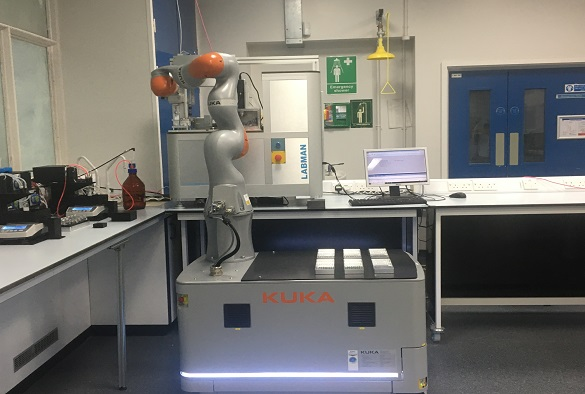
\includegraphics[width=\linewidth,height=31mm,keepaspectratio]{motivation_liverpool_lab.jpg}\figuregap실험실 작업 환경
      \column{.485\textwidth}\centering
      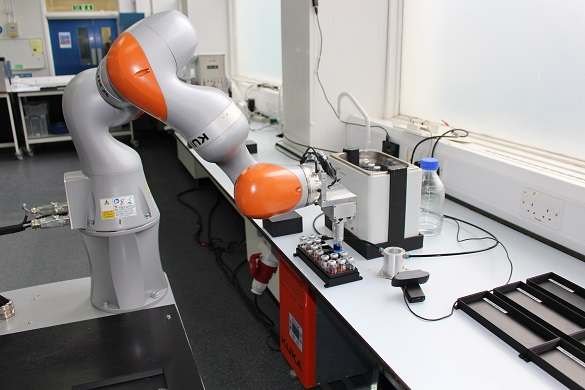
\includegraphics[width=\linewidth,height=31mm,keepaspectratio]{motivation_liverpool_handling.jpg}\figuregap시료 취급 작업
    \end{columns}\groupgap
    {\fontsize{7}{8.5}\selectfont\href{https://www.liverpool.ac.uk/cooper-group/news/stories/title,1215738,en.php}{사진 출처: 리버풀대학교}\par}\groupgap
    \textbf{안정적인 작업 수행의 전제: 충돌 없는 목표 도달}\par
  \end{slidebody}\end{frame}

\begin{frame}[label=problem]{팔 전체의 충돌 회피와 목표 도달}
  \framesubtitle{2.1 시스템 모델과 제어 목표}
  \begin{slidebody}
    \planarstage{progressive_planar_02_scene_labeled.pdf}{%
      \textbf{3자유도 planar 기구학 모델}~\slidecite{siciliano2009robotics}\detailgap
      $\dot q=u,\quad q,u\in\mathbb R^3$\detailgap
      $q$: 관절각,\quad $u$: 관절 속도 입력\groupgap
      \textbf{Task: 로봇이 달성해야 하는 제어 목표}\detailgap
      본 연구: End-effector의 목표 pose 도달\detailgap
      위치 $p_3\to p_d$, yaw $\psi_3\to\psi_d$\groupgap
      \textbf{이동 과정의 안전 제약}\detailgap
      장애물과 자기충돌 회피, 관절각 제한}
  \end{slidebody}\end{frame}

\defensepart{Background}
\begin{frame}[label=safety]{안전 제약: Control Barrier Function (CBF)}
  \framesubtitle{2.2 안전 제약 조건 설계}
  \begin{slidebody}\centering
    \textbf{Capsule로 모델링한 링크와 원형 장애물}\groupgap
    \begin{columns}[c,onlytextwidth]
      \column{.47\textwidth}\centering
      \begin{tikzpicture}[x=9mm,y=9mm]
        \path[use as bounding box](-.3,-.65)rectangle(5.3,3.65);
        \fill[EmphasisGreen!16,even odd rule](-.3,-.65)rectangle(5.3,3.65)(3.8,1.65)circle(1.05);
        \draw[line width=3.3mm,line cap=round,Accent!40](.83,.35)--(.83,2.95);
        \draw[line width=1pt,Accent](.83,.35)--(.83,2.95);
        \filldraw[fill=black!14,draw=black!65](3.8,1.65)circle(.6);
        \draw[dashed,EmphasisGreen,thick](3.8,1.65)circle(1.05);
        \draw[<->,thick](1.01,1.65)--node[above]{$d(q)$}(3.2,1.65);
        \draw[<->,EmphasisGreen,thick](3.8,2.25)--(3.8,2.70);
        \node[text=EmphasisGreen,anchor=west]at(3.92,2.46){$m_o$};
        \node[text=EmphasisBlue]at(.83,3.5){링크};
        \node at(3.8,.12){장애물};
        \node[text=EmphasisGreen]at(2.55,3.32){경계 $h=0$};
        \draw[EmphasisGreen](2.85,3.1)--(3.25,2.55);
        \node[text=EmphasisGreen,anchor=west]at(0,-.3){안전 집합 $\mathcal C$};
      \end{tikzpicture}
      \column{.49\textwidth}\raggedright
      \hspace*{3mm}\begin{tabular}{@{}l@{}}
        \textbf{안전 여유를 반영한 거리}                  \\[\SlideDetailGap]
        $h(q)=d(q)-m_o$                         \\[\SlideGroupGap]
        \textbf{CBF 제약}~\slidecite{ames2017cbf} \\[\SlideDetailGap]
        $\dot h=\nabla_qh^\top u\geq-\gamma h$  \\[\SlideGroupGap]
        \textbf{경계에서의 조건}                       \\[\SlideDetailGap]
        $h=0\ \Rightarrow\ \dot h\geq0$
      \end{tabular}
    \end{columns}\groupgap
    $\mathcal C=\{q\mid h_r(q)\geq0,\quad\forall r\text{ (모든 안전 제약)}\}$\par
  \end{slidebody}\end{frame}

\begin{frame}[label=direct-qp]{CLF--CBF QP 기반 목표 추종}
  \framesubtitle{2.3 단일 QP 기반 기구학 제어기}
  \begin{slidebody}\centering
    % Separate the CLF definition from the optimization problem visually.
    % Local padding keeps both boxes within the existing slide body.
    \setlength{\SlideMathRowGap}{.5mm}
    \setlength{\SlideGroupGap}{2mm}
    \setlength{\fboxsep}{1.2mm}
    \setlength{\fboxrule}{.5pt}
    \fcolorbox{Accent!60}{white}{%
      \begin{minipage}{\dimexpr\linewidth-2\fboxsep-2\fboxrule\relax}\centering
        \textcolor{EmphasisBlue}{Control Lyapunov Function (CLF)}\groupgap
        $V(q)=w_v\norm{p_3-p_d}^2+w_\psi[1-\cos(\psi_3-\psi_d)]$\par
      \end{minipage}}\groupgap
    \fcolorbox{Accent!60}{white}{%
      \begin{minipage}{\dimexpr\linewidth-2\fboxsep-2\fboxrule\relax}\centering
        \textbf{이차계획법 (QP)}: 목표 추종과 안전 제약의 조정~\slidecite{ames2017cbf}\groupgap
        $\begin{alignedat}{2}
        \min_{u,\delta}\quad & \tfrac12u^\top Wu+\tfrac12w_\delta\delta^2
                             &\quad & \\[\SlideMathRowGap]
        \text{s.t.}\quad     & \textcolor{EmphasisBlue}{\dot V=\nabla_qV^\top u\leq-cV+\delta}
                             &\quad & \textcolor{EmphasisBlue}{\text{CLF 제약}} \\[\SlideMathRowGap]
                             & \textcolor{EmphasisGreen}{\dot h_r=\nabla_qh_r^\top u\geq-\gamma_rh_r}\quad\forall r
                             &\quad & \textcolor{EmphasisGreen}{\text{CBF 제약}} \\[\SlideMathRowGap]
                             & u_{j,\min}\leq u_j\leq u_{j,\max},\quad j=1,2,3
                             &\quad & \text{관절 속도 제한}
          \end{alignedat}$\groupgap
        $\delta$: CLF 완화변수\qquad $W\succ0,\ c,w_\delta,w_v,w_\psi>0$\par
      \end{minipage}}\groupgap
    \textcolor{EmphasisBlue}{\textbf{Direct 제어: 최종 end-effector pose를 처음부터 추종}}\par
  \end{slidebody}\end{frame}

\begin{frame}[label=limitation]{Direct 제어가 실패할 수 있는 이유}
  \framesubtitle{2.4 순차적 기구학 제어기: 제안 배경}
  \begin{slidebody}\centering
    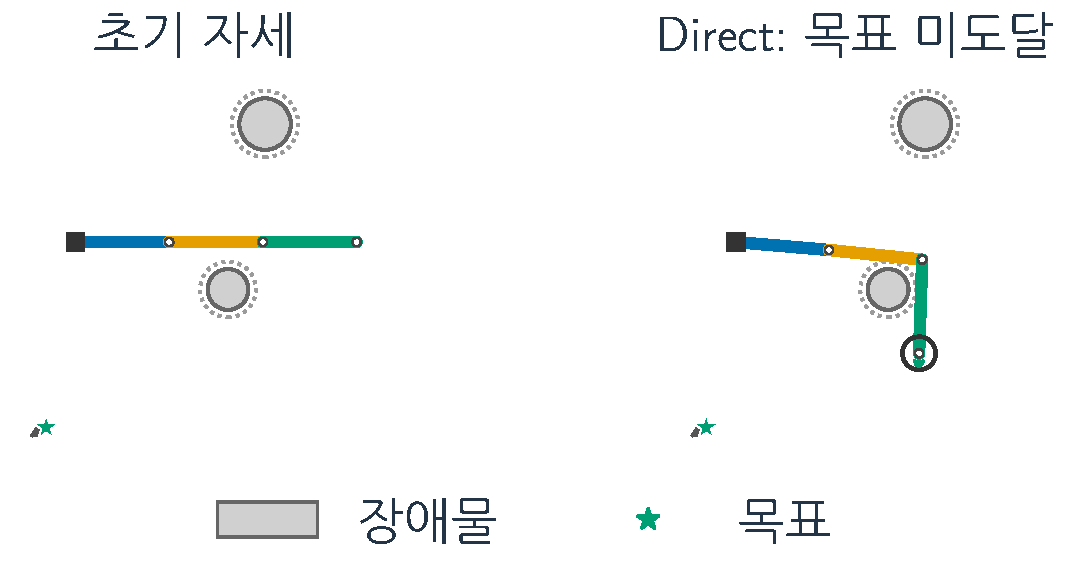
\includegraphics[width=\linewidth,height=37mm,keepaspectratio]{concept_planar_direct.pdf}\figuregap
    \textbf{CLF--CBF QP를 통한 목표 추종에도 목표 미도달 가능}\groupgap
    이론적 배경: CBF 기반 QP의 비목표 평형점~\slidecite{tan2024equilibria}\groupgap
    \textcolor{EmphasisBlue}{\textbf{최종 목표를 추종하기 전에,}}\\
    어떤 하위 작업 (subtask)을 수행하면 목표 도달에 도움이 되는가?
  \end{slidebody}\end{frame} 

\begin{frame}[label=related-work]{선행 연구와 본 연구의 설계 초점}
  \framesubtitle{1 서론}
  \begin{slidebody}
    \begin{tabularx}{\linewidth}{@{}>{\raggedright\arraybackslash}p{38mm}>{\raggedright\arraybackslash}X@{}}
      \textbf{연구} & \textbf{설계 초점}                                             \\\midrule
      Mansard \& Chaumette\newline
      (2007)~\slidecite{mansard2007sequencing}
                  & \textbf{Task 활성화·해제}\detailgap
      제약에 대응하도록 task 구성 조정                                                     \\[\SlideGroupGap]
      Basso \& Pettersen\newline
      (2020)~\slidecite{basso2020priority}
                  & \textbf{Task 우선순위 보존}\detailgap
      상위 task의 성능을 보존하며 다른 task 수행                                             \\[\SlideGroupGap]
      \textcolor{EmphasisBlue}{\textbf{본 연구}}
                  & \textcolor{EmphasisBlue}{\textbf{Subtask 목표 구성}}\detailgap
      목표 역기구학 (IK) 해에서 링크별 위치 목표 생성
    \end{tabularx}\groupgap
    \begin{beamercolorbox}[sep=2mm,wd=\linewidth]{block body}
      \textcolor{EmphasisBlue}{\textbf{목표 IK의 팔 배치를 활용하여,}}\\
      목표 도달을 돕는 링크 subtask를 구성할 수 있는가?
    \end{beamercolorbox}\par
  \end{slidebody}\end{frame}

\defensepart{Method}
\begin{frame}[label=ik]{제안 방법: IK에서 링크 목표 구성}
  \framesubtitle{2.4 순차적 기구학 제어기}
  \begin{slidebody}
    \planarstage{progressive_planar_03_ik.pdf}{%
      \textbf{충돌 없는 목표 configuration $q^*$}\detailgap
      $p_3(q^*)=p_d,\quad\psi_3(q^*)=\psi_d$\groupgap
      \textbf{Subtask: 단계별 제어 목표}\detailgap
      최종 목표 도달을 돕는 링크 끝점 제어\detailgap
      목표 $p_i^*=p_i(q^*),\quad i=1,2$\groupgap
      \textcolor{EmphasisBlue}{\textbf{Sequential: subtask의 순차 실행}}\detailgap
      링크 1 $\to$ 링크 2 $\to$ end-effector\groupgap
      점선: IK 자세\quad 별: 목표 위치}
  \end{slidebody}\end{frame}

\begin{frame}[label=stage1]{Sequential 1단계: 링크 1의 끝점 위치}
  \framesubtitle{2.4 순차적 기구학 제어기}
  \begin{slidebody}
    \planarstage{progressive_planar_04_link1.pdf}{%
      \stagechain{1}\groupgap
      \textcolor{EmphasisBlue}{\textbf{링크 1 끝점의 CLF: $V_1$}}\detailgap
      $V_1(q)=w_v\norm{p_1-p_1^*}^2$\detailgap
      $\dot V_1\leq-c_1V_1+\delta$\groupgap
      안전 제약과 관절 속도 제한 유지\detailgap
      End-effector 오차는 증가할 수 있음}
  \end{slidebody}\end{frame}

\begin{frame}[label=stage2]{Sequential 2단계: 링크 2의 끝점 위치}
  \framesubtitle{2.4 순차적 기구학 제어기}
  \begin{slidebody}
    \planarstage{progressive_planar_05_link2.pdf}{%
      \stagechain{2}\groupgap
      \textcolor{EmphasisOrange}{\textbf{링크 2 끝점의 CLF: $V_2$}}\detailgap
      $V_2(q)=w_v\norm{p_2-p_2^*}^2$\detailgap
      $\dot V_2\leq-c_2V_2+\delta$\groupgap
      안전 제약과 관절 속도 제한 유지\detailgap
      새로운 링크 목표에 따른 팔의 재배치}
  \end{slidebody}\end{frame}

\begin{frame}[label=stage3]{Sequential 최종 단계: End-effector pose}
  \framesubtitle{2.4 순차적 기구학 제어기}
  \begin{slidebody}
    \planarstage{progressive_planar_06_ee.pdf}{%
      \stagechain{3}\groupgap
      \textcolor{EmphasisGreen}{\textbf{최종 subtask: 원래의 pose 목표}}\detailgap
      $V_3(q)\equiv V(q),\quad c_3=c$\detailgap
      $\dot V_3\leq-c_3V_3+\delta$\groupgap
      안전 제약과 관절 속도 제한 유지\detailgap
      Direct와 동일한 최종 CLF}
  \end{slidebody}\end{frame}

\begin{frame}[label=clf-switch]{각 단계에서 하나의 CLF만 활성화}
  \framesubtitle{2.4 순차적 기구학 제어기}
  \begin{slidebody}\centering
    \begin{tikzpicture}[x=1mm,y=1mm]
      \path[use as bounding box](0,-28)rectangle(118,10);
      \foreach \x/\i/\col in {19/1/EmphasisBlue,59/2/EmphasisOrange,99/3/EmphasisGreen}{%
          \node[text=\col,font=\bfseries](q\i)at(\x,6){$\mathrm{QP}_{\i}$};}
      \foreach \x/\i/\col in {19/1/EmphasisBlue,59/2/EmphasisOrange}{%
      \begin{scope}[shift={(\x,-12)},x=7mm,y=3.4mm]
        \draw[-{Stealth}](-2,0)--(2,0);
        \draw[-{Stealth}](0,0)--(0,3.1)node[above]{$V_{\i}$};
        \draw[\col,thick,domain=-1.8:1.8,samples=50]plot(\x,{.7*\x*\x});
      \end{scope}
      \node at(\x,-17){위치 오차};
      \node at(\x,-25){$\dot V_{\i}\leq-c_{\i}V_{\i}+\delta$};}
      \begin{scope}[shift={(89,-12)},x=3.5mm,y=3.4mm]
        \draw[-{Stealth}](-2,0)--(2,0);\draw[-{Stealth}](0,0)--(0,3);
        \draw[EmphasisGreen,thick,domain=-1.8:1.8,samples=50]plot(\x,{.7*\x*\x});
      \end{scope}
      \node at(98,-9){$+$};
      \begin{scope}[shift={(109,-12)},x=2.2mm,y=3.4mm]
        \draw[-{Stealth}](-3.6,0)--(3.6,0);\draw[-{Stealth}](0,0)--(0,3);
        \draw[EmphasisGreen,thick,domain=-3.14:3.14,samples=50]plot(\x,{1-cos(\x r)});
      \end{scope}
      \node at(89,-17){위치};\node at(109,-17){yaw};
      \node at(99,-25){$\dot V_3\leq-c_3V_3+\delta$};
      \draw[arr](q1.east)--node[above=1mm]{단계 전환}(q2.west);
      \draw[arr](q2.east)--node[above=1mm]{단계 전환}(q3.west);
    \end{tikzpicture}\groupgap
    \textcolor{EmphasisBlue}{\textbf{단계 전환 시 이전 링크의 CLF 제약 해제}}\groupgap
    \textbf{전환 조건: subtask 목표 도달 또는 정체 감지}\groupgap
    매 제어 주기 하나의 QP 계산. 안전 제약과 관절 속도 제한은 유지\par
  \end{slidebody}\end{frame}

\begin{frame}[label=mechanism]{링크 subtask가 도움이 되는 이유}
  \framesubtitle{2.4 순차적 기구학 제어기: 설계 근거}
  \begin{slidebody}\centering
    \setlength{\SlideGroupGap}{2mm}
    \textbf{낮은 차원의 목표로 팔을 재배치할 여지 확보}\groupgap
    \renewcommand{\arraystretch}{1.12}
    \begin{tabular}{lcc}\toprule
      제어 목표 $x_i$ & $\operatorname{rank}J_i$ & Null-space 차원 \\\midrule
      링크 1 끝점 위치 $x_1=p_1$ & 1 & \textcolor{EmphasisBlue}{2} \\
      링크 2 끝점 위치 $x_2=p_2$ & 2 & \textcolor{EmphasisOrange}{1} \\
      End-effector pose $x_3=(p_3^\top,\psi_3)^\top$ & 3 & 0 \\\bottomrule
    \end{tabular}\groupgap
    $J_i(q)=\dfrac{\partial x_i}{\partial q},\qquad
      \textcolor{EmphasisBlue}{\nabla_q V_i=J_i^\top\nabla_{x_i}V_i}$\groupgap
    \begin{tikzpicture}[x=1mm,y=1mm]
      \node[box,text width=29mm,inner ysep=2mm](a)at(18,0){링크 끝점 위치\\subtask};
      \node[box,text width=29mm,inner ysep=2mm](b)at(59,0){팔의 배치\\변경};
      \node[box,text width=29mm,inner ysep=2mm](c)at(100,0){최종 pose\\제어};
      \draw[arr](a)--(b);\draw[arr](b)--(c);
    \end{tikzpicture}\groupgap
    안전, 입력 제약을 적용하지 않고 특이점을 제외한 \textbf{task Jacobian $J_i$ 기준}.
  \end{slidebody}\end{frame}

\defensepart{Results}
\begin{frame}[label=setup]{모의실험 조건과 성공 기준}
  \framesubtitle{2.5 모의실험 결과}
  \begin{slidebody}
    \begin{columns}[c,onlytextwidth]
      \column{.43\textwidth}\centering
      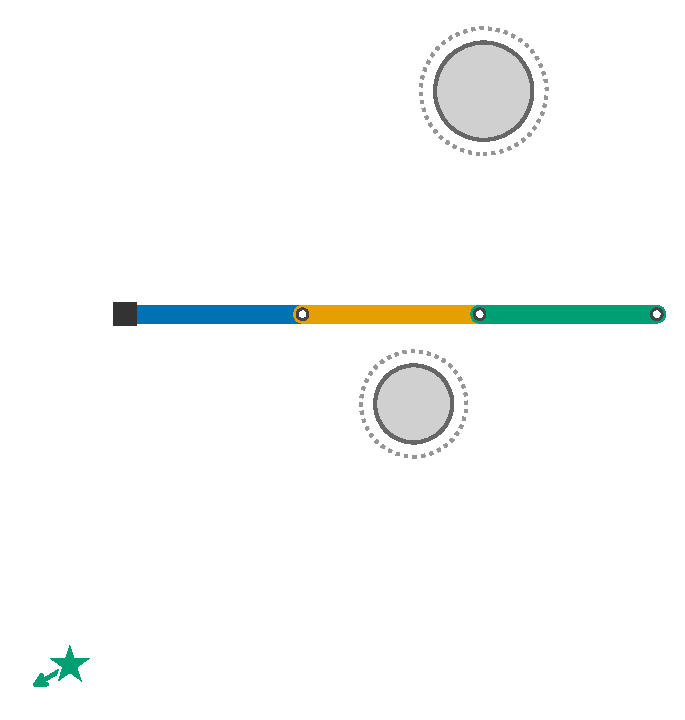
\includegraphics[width=\linewidth,height=38mm,keepaspectratio]{progressive_planar_02_scene.pdf}
      \column{.54\textwidth}
      \textbf{유효한 IK를 가진 300개 episode}\detailgap
      길이 1 m인 링크 3개, 원형 장애물 2개\detailgap
      초기 관절각 $q_0=(0,0,0)$\detailgap
      목표 pose와 장애물 배치의 무작위 생성\detailgap
      제한 시간 $T=35$ s
    \end{columns}\groupgap
    \centering\textbf{성공 기준}\detailgap
    위치 오차 $\leq0.1$ m\quad yaw 오차 $\leq0.1$ rad\detailgap
    충돌 관련 장벽함수의 최솟값 $\geq-0.01$ m\par
  \end{slidebody}\end{frame}

\begin{frame}[label=results]{목표 도달 성공률의 향상}
  \framesubtitle{2.5 모의실험 결과}
  \begin{slidebody}\centering
    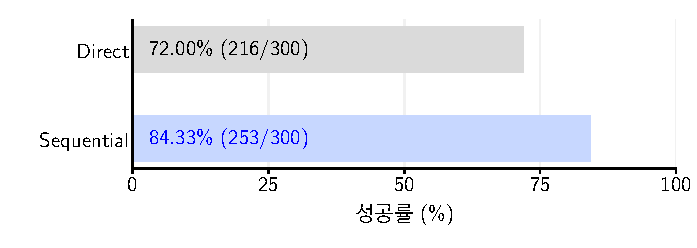
\includegraphics[width=\linewidth,height=42mm,keepaspectratio]{cics_success.pdf}\figuregap
    \textcolor{EmphasisBlue}{\textbf{Direct 대비 성공률 12.33\%p 향상}}\groupgap
    시간 초과: 65 $\to$ 36개 episode\par
  \end{slidebody}\end{frame}

\begin{frame}[label=trajectories]{Subtask 전환을 통한 목표 도달 사례} 
  \framesubtitle{2.5 모의실험 결과}
  \begin{slidebody}\centering
    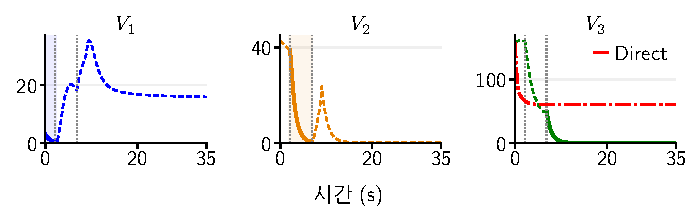
\includegraphics[width=\linewidth,height=29mm,keepaspectratio]{cics_clf_time.pdf}\figuregap
    실선: 활성 CLF\qquad 점선: 비활성 CLF\groupgap
    \textbf{비활성 task의 오차는 증가할 수 있음}\detailgap
    Sequential: 18.226 s에 최종 pose 도달\detailgap
    Direct: 같은 episode에서 목표 오차가 남음\par
  \end{slidebody}\end{frame}

\defensepart{Closing}
\begin{frame}[label=conclusion]{결론}
  \framesubtitle{3 결론}
  \begin{slidebody}
    \textbf{IK에서 링크 목표 구성}\detailgap
    하나의 목표 IK에서 두 링크의 끝점 목표 추출\groupgap
    \textbf{Sequential QP 제어}\detailgap
    최종 pose 제어 전, 일시적인 subtask의 순차 실행\groupgap
    \textbf{평가한 episode에서 성공률 향상}\detailgap
    동일한 300개 episode에서 72.00\% $\to$ 84.33\%\groupgap
    \begin{beamercolorbox}[sep=2mm,wd=\linewidth]{block body}
      \textbf{한계:} Direct만 성공한 10개 episode 존재\detailgap
      전역 수렴 보장 없음
    \end{beamercolorbox}\groupgap
    \textbf{후속 연구:} 3차원 다자유도 로봇팔로 확장\par
  \end{slidebody}\end{frame}

\begin{frame}[c,label=thanks]{}
  \centering{\fontsize{32}{38}\selectfont\textcolor{Accent}{감사합니다}}
\end{frame}

\appendix
\begin{frame}[label=appendix-contents]{부록 목차}
  \framesubtitle{보충 자료}
  \hypertarget{appendix-contents}{}
  \begin{slidebody}\vfill
    \hyperlink{app-safety}{A1. 충돌 회피와 관절각 제한}\par\vfill
    \hyperlink{app-ik}{A2. IK 선택과 단계 전환}\par\vfill
    \hyperlink{app-qp}{A3. 단계별 QP와 CLF 계수}\par\vfill
    \hyperlink{app-evidence}{A4. 동일 episode의 성공·실패 비교}\par\vfill
    \hyperlink{app-paper}{A5. CICS 제출 원고의 그림}\par\vfill
    \hyperlink{app-refs}{A6. 참고문헌}\par\vfill
  \end{slidebody}\end{frame}

\begin{frame}[label=app-safety]{A1. 충돌 회피와 관절각 제한}
  \framesubtitle{2.2 안전 제약 조건 설계}
  \begin{slidebody}\centering
    \textbf{Capsule 반지름 $\rho$; 장애물 중심 $c_j$, 반지름 $r_j$}\detailgap
    $h_{ij}^{\rm obs}=\operatorname{dist}(c_j,[p_{i-1},p_i])-\rho-r_j-m_o$\groupgap
    \textbf{길이가 같은 링크의 자기충돌 모델}\detailgap
    $h_1^{\rm link}=\operatorname{dist}(p_3,[p_0,p_1])-\rho-m_\epsilon$\detailgap
    $h_2^{\rm link}=\operatorname{dist}(p_0,[p_2,p_3])-\rho-m_\epsilon$\groupgap
    \textbf{관절각 제한}\detailgap
    $h_j^-=q_j-q_{j,\min},\quad h_j^+=q_{j,\max}-q_j$\groupgap
    \textbf{모든 장벽함수를 인덱스 $r$로 표기}\detailgap
    $\nabla_qh_r^\top u\geq-\gamma_rh_r,\qquad\gamma_r>0$\par
  \end{slidebody}\end{frame}

\begin{frame}[label=app-ik]{A2. IK 선택과 단계 전환}
  \framesubtitle{2.4 순차적 기구학 제어기}
  \begin{slidebody}\centering
    \textbf{목표와 안전 조건을 만족하는 IK 후보}\detailgap
    $p_3(q)=p_d,\quad\psi_3(q)=\psi_d,\quad h_r(q)\geq0\quad\forall r$\groupgap
    $q^*\in\argmin_{q\in\mathcal Q_{\rm valid}}\norm{\operatorname{wrap}(q-q_0)}$\detailgap
    $\mathcal Q_{\rm valid}$: 안전 제약을 만족하는 IK 후보 집합\groupgap
    $p_i^*=p_i(q^*),\quad i=1,2$\groupgap
    \textbf{링크 1·2 단계}\detailgap
    목표 도달 또는 정체 감지 시 다음 단계로 전환\groupgap
    \textbf{최종 단계}\detailgap
    원래의 end-effector pose 추종; $q^*$ 도달은 요구하지 않음\par
  \end{slidebody}\end{frame}

\begin{frame}[label=app-qp]{A3. 단계별 QP}
  \framesubtitle{2.3--2.4 QP 기반 제어기}
  \begin{slidebody}\centering
    $\begin{aligned}
        (u_i^*,\delta_i^*) & =\argmin_{u,\delta}\ \tfrac12u^\top Wu+\tfrac12w_\delta\delta^2 \\[\SlideMathRowGap]
        \text{s.t.}\quad   & \nabla_qV_i^\top u\leq-c_iV_i+\delta,                           \\[\SlideMathRowGap]
                           & \nabla_qh_r^\top u\geq-\gamma_rh_r\quad\forall r,               \\[\SlideMathRowGap]
                           & u_{j,\min}\leq u_j\leq u_{j,\max},\quad j=1,2,3.
      \end{aligned}$\groupgap
    $V_i=w_v\norm{p_i-p_i^*}^2,\quad i=1,2$\detailgap
    $V_3=w_v\norm{p_3-p_d}^2+w_\psi[1-\cos(\psi_3-\psi_d)]$\groupgap
    \textbf{제출 원고의 사례: $w_v=10$, $w_\psi=5$}\detailgap
    저장된 구현의 표현: $10[\norm{e_p}^2+0.5(1-\cos e_\psi)]$\par
  \end{slidebody}\end{frame}

\begin{frame}[label=app-evidence]{A4. 동일 episode의 성공·실패 비교}
  \framesubtitle{2.5 모의실험 결과}
  \begin{slidebody}\centering
    \begin{tabular}{lrr}\toprule
                & Sequential 성공 & Sequential 실패 \\\midrule
      Direct 성공 & 206           & 10            \\
      Direct 실패 & 47            & 37            \\\bottomrule
    \end{tabular}\groupgap
    \textbf{동일한 300개 episode에서 성공 건수 37개 증가}\groupgap
    \begin{tabular}{lrr}\toprule
      실패 유형     & Direct & Sequential \\\midrule
      시간 초과     & 65     & 36         \\
      QP 실행 불가능 & 17     & 10         \\
      안전 기준 위반  & 2      & 1          \\\bottomrule
    \end{tabular}\groupgap
    모의실험에서 개선 확인; 전역 수렴 보장 없음\par
  \end{slidebody}\end{frame}

\begin{frame}[label=app-paper]{A5. CICS 제출 원고의 그림}
  \framesubtitle{2.5 모의실험 결과}
  \centering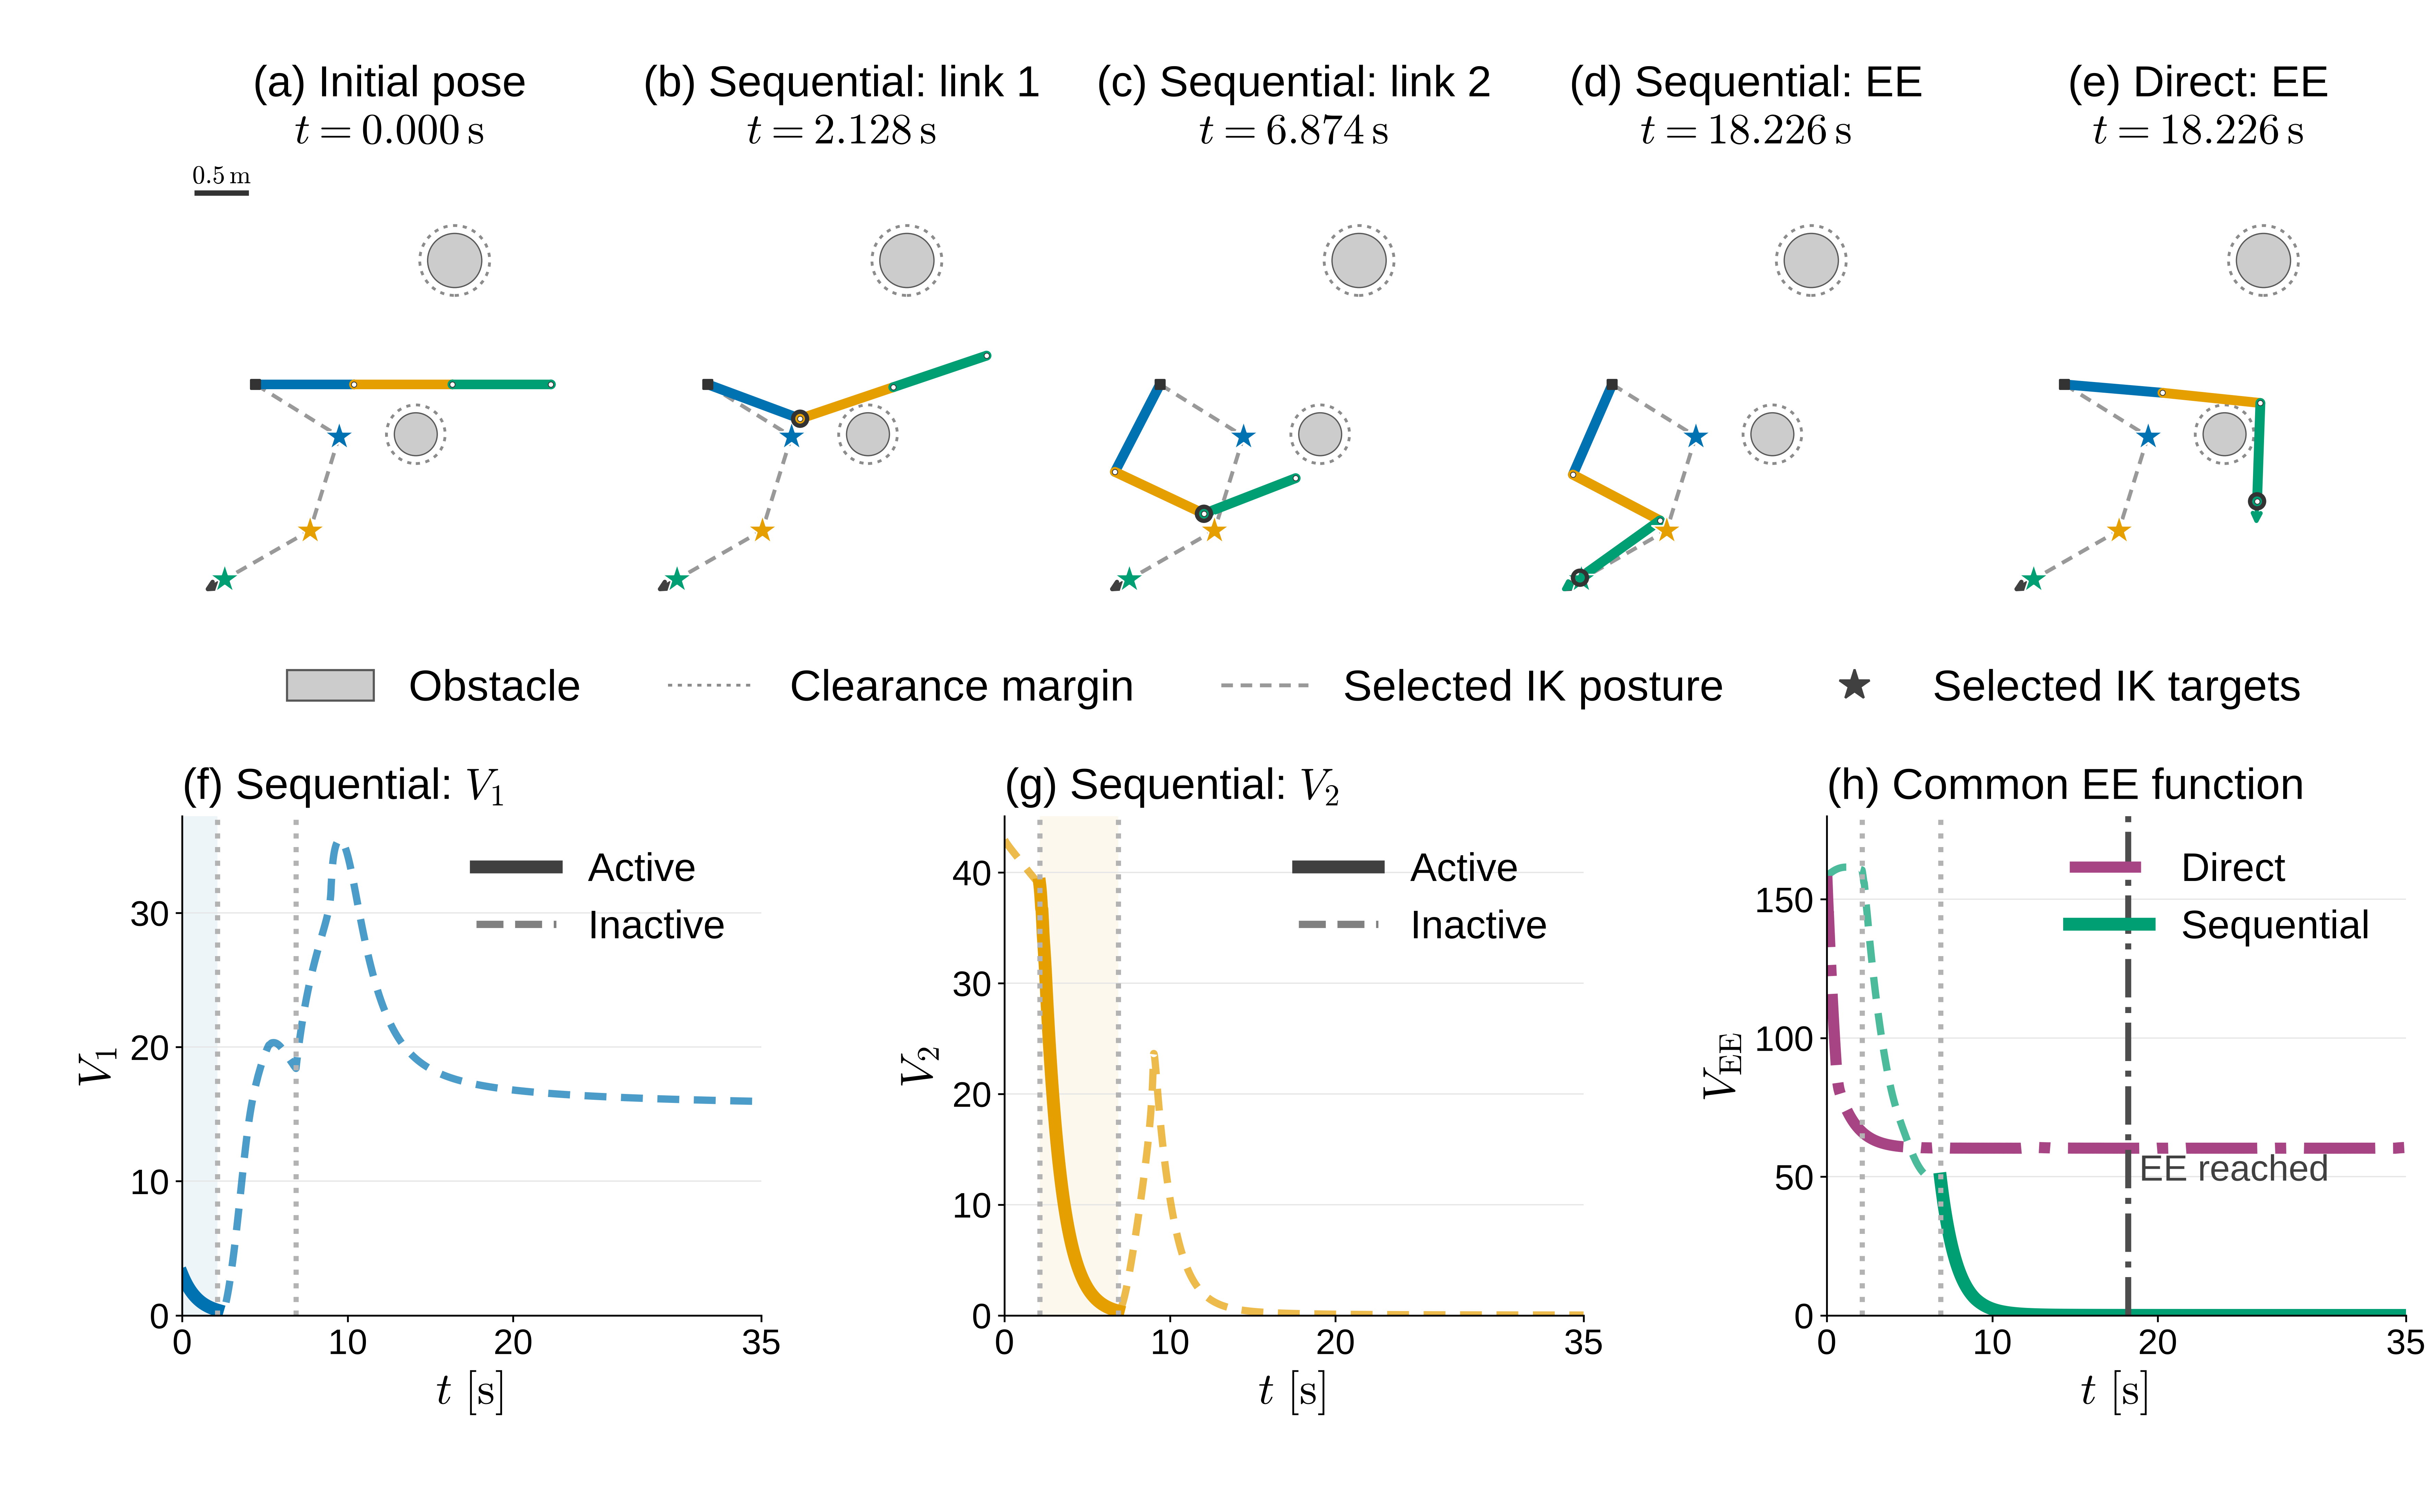
\includegraphics[width=\linewidth,height=57.5mm,keepaspectratio]{source/BIN0002.png}
\end{frame}

% A separate anchor preserves navigation without truncating frame continuations.
\begin{frame}[allowframebreaks]{A6. 참고문헌}
  \framesubtitle{제출 원고·관련 연구·응용 사례의 출처}
  \hypertarget{app-refs}{}
  \bibliographystyle{IEEEtran}\bibliography{references}
\end{frame}


\end{document}

